%______________________________________________________________________

\section*{\citet{2017_Gipp}}
%______________________________________________________________________

\subsection*{Authors}
The authors of the paper can be viewed in table \ref{tab:2017_Gipp_Authors}.
\begin{longtable}{ |P{3cm}|P{4cm}|P{5cm}| }
	\caption{Authors} \label{tab:2017_Gipp_Authors} \\
	\hline
 	\cellcolor{Gray}Name & \cellcolor{Gray}Location & \cellcolor{Gray}Institution \\ [0.5ex] 
 	\hline\hline
 	\endhead
	 Bela Gipp &  \multirow{3}{4cm}{\centering Konstanz, Germany} & \multirow{3}{5cm}{\centering University Of Konstanz} \\
	 \cline{1-1}
	 Corinna Breitinger &  & \\
	 \cline{1-1}
	 Norman Meuschke &  & \\
	 \hline
	 Joeran Beel & Dublin, Ireland & Trinity College Dublin \\
	\hline
\end{longtable}

%______________________________________________________________________

\subsection*{Contribution}
The contribution of \citet{2017_Gipp} was a manuscript submission system called \quoteit{CryptSubmit}. It provides the functionality for academics to submit their manuscript(s), to get peer review feedback and most importantly to securely confirm the existence of research concepts, data or outcomes when a manuscript is submitted to be reviewed. Their research question is:
\begin{displayquote}
\quoteit{How can researches verify that their contribution already existed at the time of submission to a conference or journal?}
\end{displayquote}
Another contribution that they made was integrated in \quoteit{CryptSubmit} and was a service called \quoteit{OriginStamp}\urlfootnote{http://originstamp.org/}. This service can be used to create decentralized trusted timestamps on Bitcoin's Blockchain.
Their work is available open source:
\begin{enumerate}[label={\arabic*)},font={\color{red!50!black}\bfseries}]
	\item \quoteit{CryptSubmit} \url{https://www.gipp.com/cryptsubmit/}
	\item \quoteit{OriginStamp} \url{http://originstamp.org/home}
\end{enumerate}.

%______________________________________________________________________

\subsection*{Reason/Problems}
The disadvantages of current manuscript submission systems are in particular the
\begin{enumerate*}[label={\arabic*)},font={\color{red!50!black}\bfseries}]
	\item lack of standards that cause for example data leaks
	\item chance of bias and fraud during the peer-review
	\item no existance of proof, seperate of the system, to confirm the time the author's work was uploaded
\end{enumerate*}.
They stated that currently there are various trusted-timestamping systems based on Bitcoin's Blockchain, but non that adresses the issue of priority management for academic manuscripts.

%______________________________________________________________________

\subsection*{Implementation Process}
For their manuscript submission system \quoteit{CryptSubmit}, they used the \quoteit{Open Journal System (OJS)}\urlfootnote{https://openjournalsystems.com/}, which is an open-source management submission software for academic journals.
The figure \ref{fig:2017_gipp_overview} presents the architecure of \quoteit{CryptSubmit}. In their provided frontend, there are several functionalities to exploit:
\begin{enumerate*}[label={\arabic*)},font={\color{red!50!black}\bfseries}]
	\item User Registration
	\item File (e.g.\ manuscript) upload
	\item Management of peer review procedure
\end{enumerate*}.
If a person then uploads some data, a hash is automatically created by the backend of the system. This hash then gets sent to the \quoteit{OriginStamp Service}, which adds the hash onto Bitcoin's Blockchain. The service then gets the trusted timestamp back from the Blockchain and sends it to the submission system. Here the manuscript verficiation link and the trusted timestamp are presented. The person to review the paper is notified by the system, that there was an upload and also has access to verify the timestamp. The third actor in the system is the research community or simply the public. Everyone has access to the manuscript and the associated hash, so that they are able to check the time and the content of the idea that was published on the system.

\begin{figure}[!ht]
    \centering
    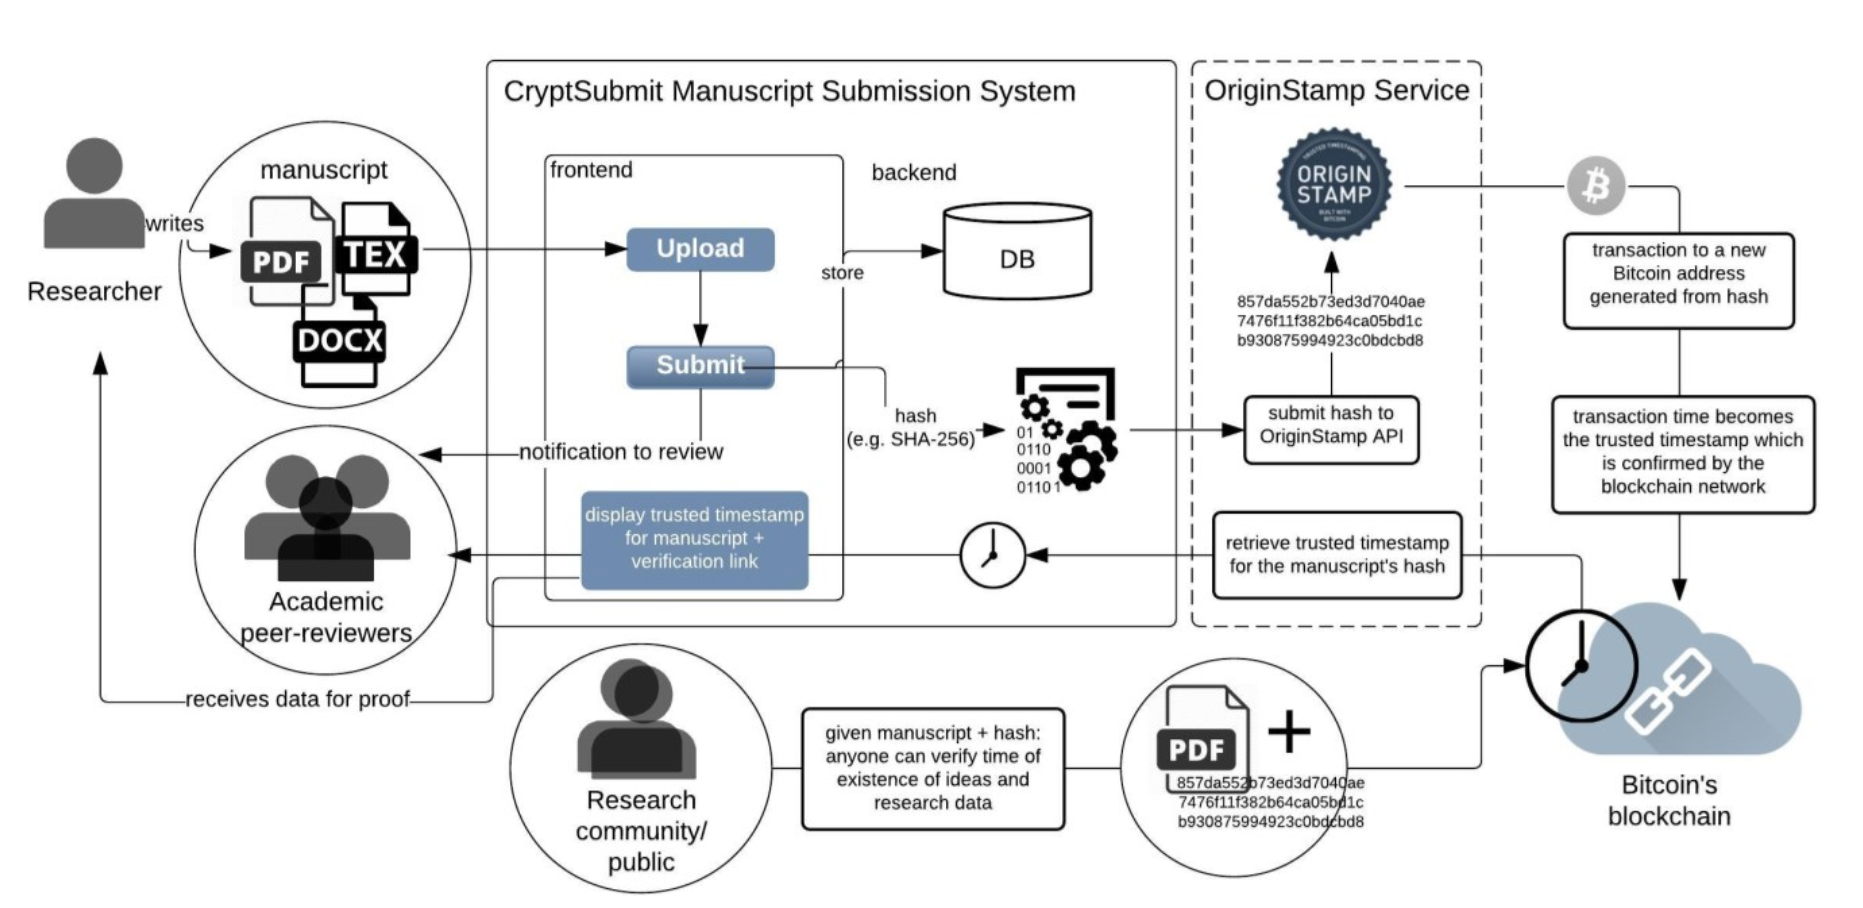
\includegraphics[width=1\textwidth]{2017_Gipp_Overview.png}
    \label{fig:2017_gipp_overview}
    \caption{Overview of the manuscript submission system implemented by \citet{2017_Gipp}}
\end{figure}

%______________________________________________________________________

\subsection*{Conclusion}
The decentralized trusted timestamp system \quoteit{OriginStamp} that they presented in the paper has a crucial advantage compared to traditional timestamp systems, there is no central timestamping authority (TSA). In the Bitcoin system this is called the Third-Trusted-Party, which represents the bank.\\
Combing the manuscript submission system which \quoteit{OriginStamp}, results in certain improvements:
\begin{itemize}
	\item Each author receives a tamperproof timestamp of when they submitted their work. This timestamp is independent of \quoteit{CrtpySubmit} system. This means, that even if someone steals the idea, the author is able to proof that he published the work first.
	\item The proposed solution will not help to fully prevent plagiarism in academia, nevertheless it will aid the researchers to justify their claim of ownership of a certain intellectual property.
	\item There are not only benefits for the authors but also for the reviewers. They are also given a proof of their feedback and can also demand to be cited for their contribution in the publication after.
\end{itemize}
For future work, they say that the approach could also be used for other submission systems and that more features of the Blockchain e.g.\ store the complete publication on the Blockchain, could be integrated.\\
